\documentclass[twoside,11pt]{homework}
\usepackage{listings}
\usepackage{xcolor}
\usepackage{graphicx} 

\coursename{COMS 4771 Machine Learning (2018 Fall)} 

\studname{Jing Qian}    % YOUR NAME GOES HERE
\studmail{jq2282@columbia.edu}% YOUR UNI GOES HERE
\hwNo{4}                   % THE HOMEWORK NUMBER GOES HERE
\date{\today} % DATE GOES HERE


\begin{document}
\maketitle

%%%%%%%%%%%%%%%%%%%%%%%%%%%%%%%%%
\section*{Problem 3}
\color{black}
\subsection*{(i)}
Let's test $purple \sim N(\left[ \begin{smallmatrix} 0\\10\end{smallmatrix}\right], 3I)$


The derivative of the discrepancy function $F = \sum_{i, j} (||x_i - x_j||-D_{i,j})^2$with respect to a location $x_i$ is:
%
\begin{equation}
\begin{split}
\frac{\partial F}{\partial x_i} &= \sum_{j} 2(x_i - x_j) - \frac{2D_{i,j}}{||x_i - x_j||}(x_i - x_j) \\
&=\sum_{j} 2(1-\frac{D_{i,j}}{||x_i - x_j||})(x_i - x_j) 
\end{split}
\label{E31}
\end{equation}
 %
 
 \newpage
 \subsection*{iii}
 To minimize the discrepancy function, we want to find the point where the derivative Eq.~\ref{E31} in equal to zero.
 Here we use the Batch Gradient Descent method considering we only have 9 data points.
 We set the initial locations of every city as a 2-d vector with random values.
In Fig.~\ref{EstiLoc}, we set $\alpha = 0.05$ and iteration number to 10000.
When increasing the iteration number, the result doesn't vary much.
And the result remains similar when $\alpha $ set to 0.1 or 0.01.
So  $\alpha = 0.05$  and 10000 iterations are good enough input parameters.

From the estimated locations, we could calculate the discrepancy funciton $F = \sum_{i, j} (||x_i - x_j||-D_{i,j})^2 = 908467$.

In Fig.~\ref{EstiLoc}, the distribution of the nine cities are quite similar to their locations in the US map.
But this is not always the case, sometimes we get the rotated distribution while keeping the relative locations.
This is because the input is the distance between different cities, not the difference between the location vectors of cities.
As a result, estimated locations would get a good prediction of the shape of the distributions, not their exactly 2-d value in the map.

 %
%%%%%%%%%%%%%%%%%%% Fig. 1 %%%%%%%%%%%%%%%%%%%%%%%%%%%%%%
\begin{figure}[ht]
\centering
\includegraphics[]{EstimatedLocation.pdf}
%\includegraphics[]{figs/EstimatedLocation.pdf}
\caption{Estimated location from Batch Gradient Descent method.}
\label{EstiLoc}
\end{figure}
%%%%%%%%%%%%%%%%%%%%%%%%%%%%%%%%%%%%%%%%%%%%%%%%%%%
%
\end{document} 
